%%%%%%%%%%%%%%%%%%%%%%%%%%%%%%%%%%%%
%% PREAMBLE 
%%%%%%%%%%%%%%%%%%%%%%%%%%%%%%%%%%%%

\documentclass[11pt]{article}

% nice clickable URLs
\usepackage{url}  
\usepackage{amsmath}
\usepackage{graphicx}
\usepackage[utf8]{inputenc}
\usepackage[english]{babel}
\usepackage{color}
% conditional independence
\newcommand{\bigCI}{\mathrel{\text{{$\perp\mkern-10mu\perp$}}}}
\newcommand{\Sara}[1]{{\color{blue} Sara: #1}}

% page margins 
\setlength{\paperwidth}{494pt} % A4
\setlength{\textwidth}{420pt}
\setlength{\hoffset}{-30pt}
\setlength{\oddsidemargin}{-5pt}
\setlength{\paperheight}{846pt} % A4
\setlength{\textheight}{700pt}
\setlength{\voffset}{0pt}
\setlength{\topmargin}{-50pt}
\setlength{\headheight}{0pt}
\setlength{\headsep}{25pt}
\setlength{\parindent}{0pt} % {20pt}
\setlength{\parskip}{4pt plus 2pt minus 1pt}


\begin{document}

%%%%%%%%%%%%%%%%%%%%%%%%%%%%%%%%%%%%
%% HEADING 
%%%%%%%%%%%%%%%%%%%%%%%%%%%%%%%%%%%%
\rule{\textwidth}{1pt}

\textbf{Thesis Project} \hfill 2017
\rule{\textwidth}{1pt}
\vspace*{20pt}

%%%%%%%%%%%%%%%%%%%%%%%%%%%%%%%%%%%%
%% ENTER DETAILS
%%%%%%%%%%%%%%%%%%%%%%%%%%%%%%%%%%%%

% write the homework number in place of "NUM"
\textbf{Assignment 5: Project Proposal}
% This assignment requires that you write a short research proposal. Essentially a statement that specifies a research problem, and a way to arrive at a solution to that problem. The proposal should not exceed 4 pages of text (regular layout and font size). The following items should be addressed in the proposal:

% write your name(s) in place of "NAME(S)"
\textbf{Name:} Alex Khawalid, 10634207\\
\textbf{Supervisor:} Sara Magliacane\\
\today

\section{Literature Review}
Causal discovery, a field in statistics, is the cornerstone of this research. A few terms should be explained before delving further into the subject of this thesis proposal.
Causal discovery aims to uncover causal relations between random variables. In the context of causal discovery, a causal relation is some relation where given an intervention that changes X, Y changes as well. This in turn means that X causes Y.
These causal relations can be represented by causal graphs, the methods that will be presented in this these project will generate causal graphs based on a dataset.
There are two big categories of causal discovery; score-based and constraint-based. The main framework that will be discussed is part of the constraint-based type of causal discovery. Constraint-based causal discovery usually relies on a few assumptions, based on these assumptions causal graphs are generated with statistical independence tests. Using these assumptions a causal graph can be constructed from the results of the statistical independence tests. Two of these assumptions are the Markov Assumption and the Faithfulness assumption.\cite{jci}
A constraint-based method which was recently developed, produced similar accuracy results to other state of the art methods but with lower running times. This method, Ancestral Causal Inference (ACI), allows for the presence of latent variables in a system, which is true for most constraint-based methods.  ACI produces an ancestral structure, this is one of the factors that allow it to run faster than similar methods with different representations by orders of magnitude. \cite{aci}

A different method for causal discovery was proposed by Eaton and Murphy\cite{eaton2007exact}. This method is of the score-based type of causal discovery methods. In this paper Eaton and Murphy applied a technique using Dynamic Programming (DP). The result that this algorithm produces is a causal Directed Acyclical Graph (DAG). ''Exact Bayesian structure learning from uncertain interventions`` illustrates how they successfully applied this technique and what the results of their research were. \cite{eaton2007exact}
    
Yet another different method, Local Causal Discovery (LCD), can discover causal relations for a simple causal pattern. The method can also take observational and experimental data into account.\cite{cooper1999causal}

Using these different methods as a frame of reference, Joint Causal Inference (JCI) can be discussed. JCI is a framework used to discover causal relations from multiple observational and experimental datasets. JCI contains a set of assumptions which enables methods to use multiple datasets to generate a general underlying causal graph across all of the datasets. ''Joint Causal Inference from Observational and Experimental Datasets`` highlights some problems with faithfulness violations which are caused by deterministic relations from JCI. These problems are solved using an extension of ACI called Ancestral Causal Inference with Determinism (ACID). It also discusses the advantages ACID-JCI has over other methods of causal inference. Furthermore it explains that ACID-JCI allows for the structure it is learning to have latent variables. Similarly to ACI, the output model is an ancestral structure. ACID-JCI has succesfully been tested on simulated data.\cite{jci}

Since JCI has only been tested on simulated data, it will be tested on a real-world biological dataset in this thesis project.  The data that JCI will be tested on will be obtained from ''Causal Protein-Signaling Networks Derived from Multiparameter Single-Cell Data``. This paper describes the dataset which will be used and is necessary to understand it. \cite{sachs2005causal} The dataset contains data about protein concentrations after certain interventions. The purpose of applying ACID-JCI to such biological datasets is to uncover causal relations in cell signalling networks. Gaining more insight into these cell signalling networks will help in treating diseases more effectively. Understanding cell signalling networks shows how cells react to their environment and how they decide what actions to take.

The dataset being used has a rather large number of variables, ACID-JCI cannot deal with this many variables at once. The main question this thesis project will be answering is how to scale ACID-JCI.

% explain causal statistics -> causal graphs -> aci -> jci -> acid

% Literature review. Explain the state of the art regarding the research topic.


% explain jci non trivial data -> does not scale
% How to scale JCI?

% Research question. State the problem that the proposed research focusses on. This problem should follow from the literature review.

\section{Method and approach}
The proposed solution to scale ACID-JCI is as follows:
\begin{itemize}
    \item Assign overlapping subsets of variables
    \item Run ACID-JCI on subsets
    \item Combine models produced by ACID-JCI
\end{itemize}

This seems like a trivial problem to solve, however there is some difficulty involved because of the way ACID-JCI is scores its edges. ACID-JCI does not give its edges a probability, it scores its edges with a confidence score. This confidence score is an approximation and it is not normalised. This makes the combination of the causal graphs more complicated than it seems.

A baseline will be established first, this enables a simple comparison between devised methods and a baseline. Random subsets of variables will be assigned and the models produced by these subsets will be summed.

Afterwards methods of combining causal models produced by ACID-JCI will be devised and implemented. These methods of combining models will have to be theoretically sound, this however does not guarantee successful application on a real-world dataset.

When methods of combining ACID-JCI produced causal models are available, more efficient methods of assigning subsets can be looked at.

After applying and testing these methods they will be documented in the thesis. Previous research has used precision, recall and execution time to evaluate causal discovery methods.\cite{jci,aci} This research will also use precision, recall and execution time as evaluation metrics.
% explain subset and model combination -> random select baseline -> evaluate on precision recall and execution time
% Method and approach. Describe how the research will be done. What approach will be taken. 'Doing the research' often entails programming software, but there are other tasks. Maybe experiments need to be conducted. Maybe evaluation studies need to be done. Maybe more literature needs to be processed. Give a precise overview of all that is involved.
% Evaluation. Describe how the results of the research will be evaluated? In a way this can be regarded as part of the method/approach, but it is important and therefore requires independent attention. Ask the question of how proof can be realised such that the results obtained are viable. 

\section{Schedule}
The main tasks that need to be completed are as follows

\begin{itemize}
    \item \textbf{Understand codebase and get it working:} There is a working implementation of ACID-JCI available. The first task at hand is to understand how it works and get it running so it can be used.
    \item \textbf{Efficient subset assignment:} Find subsets of variables such that the causal graphs can be combined in a reasonable amount of time.
    \item \textbf{Find theoretically sound graph combination method:} When JCI is run on subsets of the data with a limited amount of variables, the resulting models have to be combined. The combination of these models has to be theoretically sound.
    \item \textbf{Apply and compare methods:} Apply the methods that were devised to scale ACID-JCI and evaluate them.
\end{itemize}

These tasks have been broken down in the Gantt chart in figure \ref{fig:my_label}.

\begin{figure}[!ht]
        \centering
        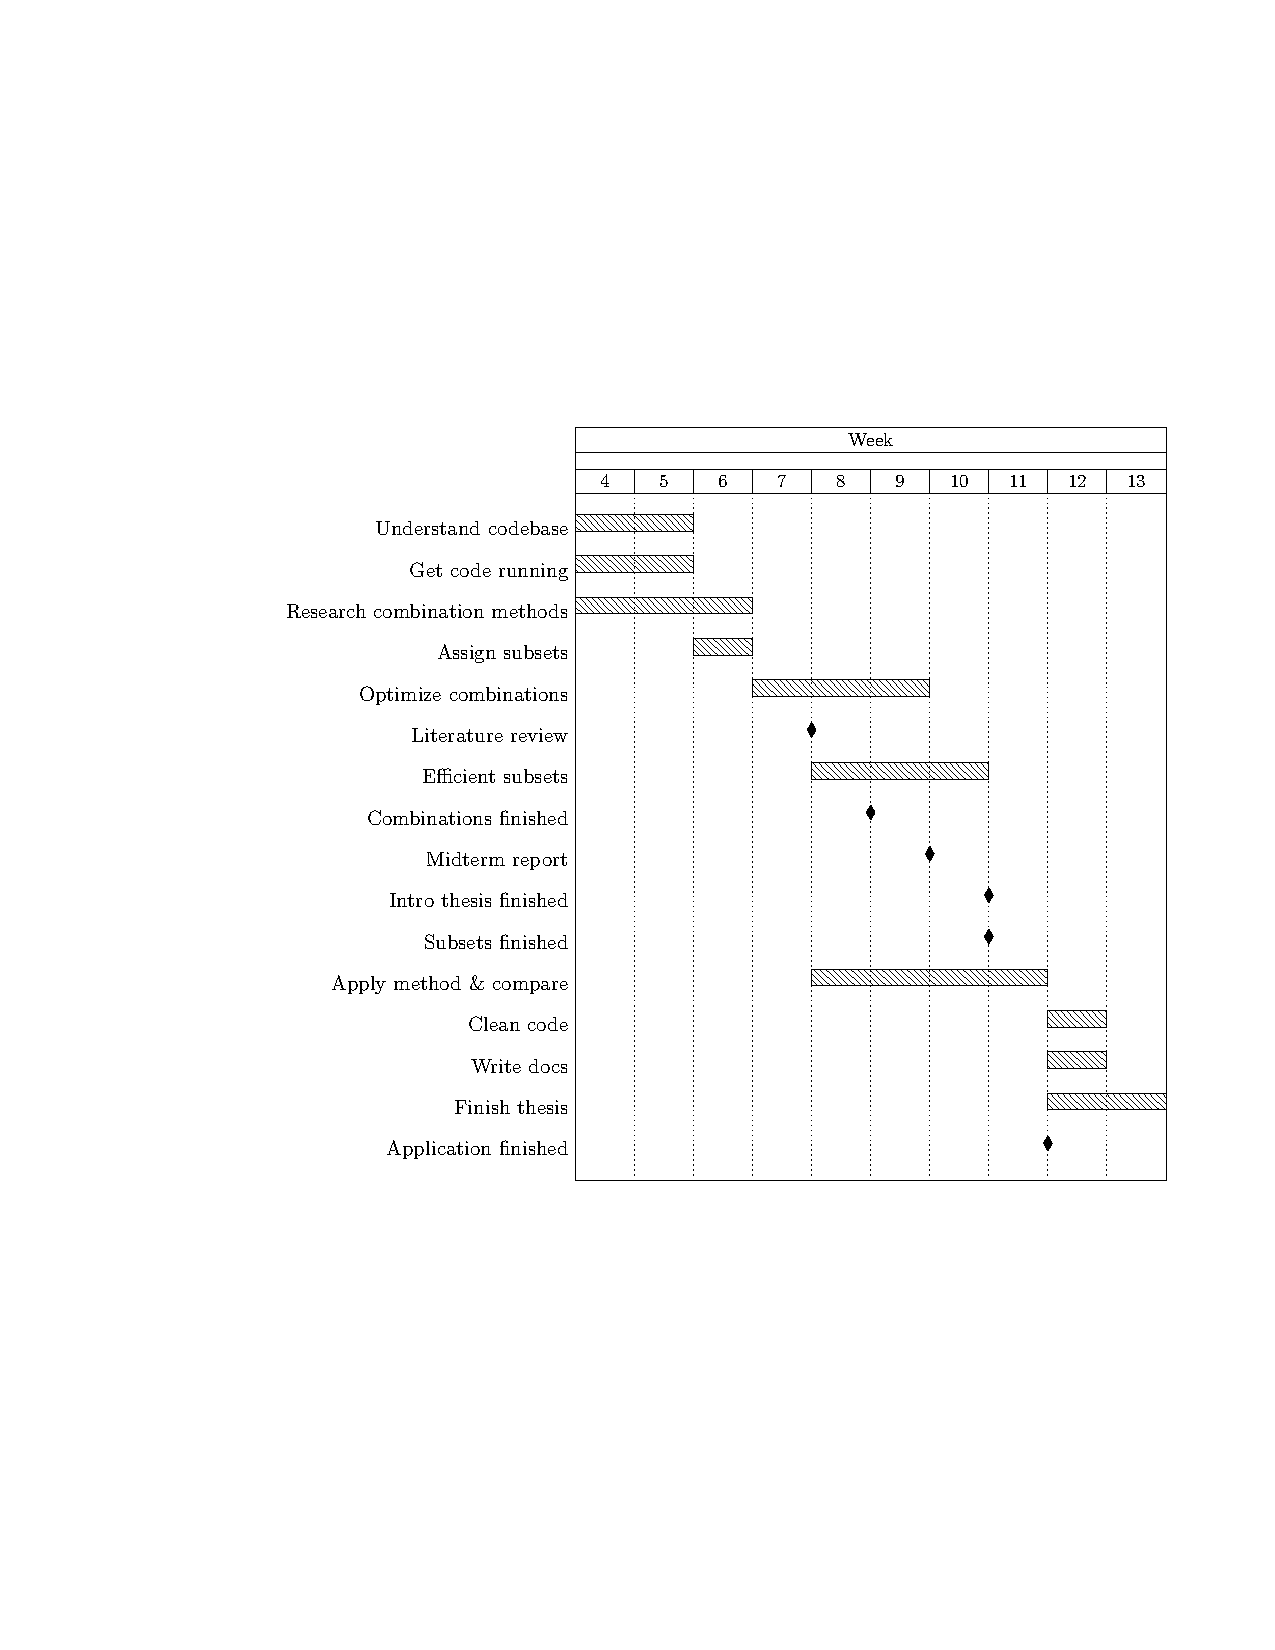
\includegraphics[width=\textwidth]{ScriptieOpdrachten.pdf}
        \caption{Schedule for thesis project}
        \label{fig:my_label}
    \end{figure}
% show gantt chart and expand on tasks and milestones

% Plan. Explicate the order in which the activities following from the above will be carried out in time. As well as how much time (effort in terms of hours or days) will be allocated to each task. A Gantt-chart is a very typical way to articulate plan. A Pert-chart  Further issues include the following. Are there multiple ways in which the activities can be organised? What are the land-marks (aka. milestones, a Pert-chart is often insightful), what decision options do these have, and on what criteria will that be evaluated? Is there a critical path? Can it become a problem? How can it be circumvented (is there a contingency plan)? 
% Report and presentations. An important output of a research project concerns the publication of the results. Allocate time in your plan to write this publication (the thesis or maybe a paper). There will also be presentations and preparing them also takes time, and hence should be part of the plan.
% Note:
% You may reuse and expand material obtained in previous assignments.
% Your kindly asked to write the proposal in English, in order for it to be of help for the Academic English class.
% This is the first result within the graduation project that will be graded. Please respect the deadline (failing the deadline with result in 0 credits for this assignment, see 'studiewijzer').
\bibliographystyle{abbrv}
\bibliography{ref1} 

\end{document}